\documentclass[10pt,twocolumn]{article}
\usepackage[margin=0.63in,columnsep=0.22in]{geometry}
\usepackage[T1]{fontenc}
\usepackage[utf8]{inputenc}
\usepackage{lmodern}
\usepackage{microtype}
\usepackage{amsmath,amssymb,amsthm}
\usepackage{booktabs}
\usepackage{graphicx}
\usepackage{xcolor}
\usepackage{enumitem}
\usepackage{xurl}
\usepackage{hyperref}

\hypersetup{
  colorlinks=true,
  linkcolor=blue!60!black,
  citecolor=blue!60!black,
  urlcolor=blue!60!black,
  pdftitle={Constructive Lean 4 Formalization and Exact-Rational Certificates for OpenAI's omega <= 9/4 Strassen Spectral Profile Proof},
  pdfauthor={Lluis Eriksson}
}

\newtheorem{proposition}{Proposition}
\newtheorem{definition}{Definition}
\newcommand{\QQ}{\mathbb{Q}}
\newcommand{\ZZ}{\mathbb{Z}}

\title{\vspace{-1.0em}\textbf{Constructive Lean~4 Formalization and Exact-Rational Certificates for OpenAI's $\omega \le 9/4$ Strassen Spectral Profile Proof}}
\author{Lluis Eriksson\thanks{Independent Researcher. Code, Lean~4 proofs, and certificates: MIT License; manuscript and figures: CC-BY-4.0. Prepared with transparent AI coding, formalization, and drafting assistance via Google Antigravity; all Lean~4 theorems, exact-$\QQ$ verifiers, and adversarial tests were independently compiled and verified locally. Repository: \href{https://github.com/lluiseriksson/openai-strassen-nine-fourths-certificates}{\nolinkurl{github.com/lluiseriksson/openai-strassen-nine-fourths-certificates}}.}}
\date{November 25, 2026}

\begin{document}
\maketitle
\vspace{-1.3em}

\begin{abstract}
OpenAI (Oct.~2, 2026) established the upper bound $\omega \le 9/4$ for the complex matrix multiplication exponent via a compact spectral-profile mechanism: finite $5M \to M$ Fourier squared-mismatch degeneration (Prop.~3.1), a determinant filtration establishing discrete concavity $2P(a,b)\ge P(a,b+1)+P(a,b-1)$ (Lem.~4.1), a three-sector decomposition giving shifted tripling $P(a,3h+a-1)\ge 3P(a,h)$ (Lem.~4.2), and an elementary discrete growth proof forcing $P(a,a)\ge a^{4/3}$ (Lem.~5.1) and thus $t \le 3/4 \implies \omega = 3t \le 9/4$. We present a standalone, zero-dependency, zero-floating-point verification stack pairing: (i)~\texttt{StrassenNineFourths.lean}, 18 constructive Lean~4.35.0 theorems (zero \texttt{sorry}, zero \texttt{axiom}, zero \texttt{Classical.choice}, zero warnings; 1 zero-axiom and 17 \texttt{[propext, Quot.sound]}) mechanizing Proposition~3.1, Lemmas~4.1--4.2, and the \emph{complete universal inductive proof} of Lemma~5.1 ($P(a,a)^3 \ge a^4$ for all $a \ge 1$) over a self-contained exact-rational structure \texttt{QRat}; and (ii)~\texttt{STRASSEN-94-CERT-1.0}, a pure-stdlib Python \texttt{Fraction} auditor across four modes. Alongside certifying 16 canonical witnesses in $0.008$--$13.686\,\mathrm{ms}$ and rejecting 60/60 live adversarial forgeries (64/64 pytest checks), our exact audit reveals a $4\times$ tightening of Proposition~3.1's degeneration degree from $(M-1)^2$ to $\lfloor(M-1)/2\rfloor^2$ (degree $0$ at $M=2$) and proves exact minimal integer refutation thresholds $a^*(t)$ for supercritical exponents $t > 3/4$.
\end{abstract}

\section{Introduction and Scope Calibration}\label{sec:intro}
Following Strassen's $2\times 2$ seven-product identity~\cite{strassen1969gaussian}, Strassen's asymptotic spectrum of tensors~\cite{strassen1988asymptotic}, and the Coppersmith--Winograd laser method~\cite{coppersmith1990matrix}, OpenAI's October~2, 2026 preprint~\cite{openai2026omega94upper} proved $\omega \le 9/4$ over $\mathbb{C}$ (complemented by a matching lower bound $\omega_F = 9/4$ in~\cite{openai2026omega94exact}) without Coppersmith--Winograd optimization tables. For any tensor character $\lambda$ with oriented dot-product exponents $p_X,p_Y,p_Z\in[0,1]$ and $t := (p_X+p_Y+p_Z)/3 > 0$, OpenAI defines the symmetrized polynomial-multiplication profile
\begin{equation}
P(a,b) := \Bigg(\prod_{\pi\in S_3} \lambda_\pi(C(a,b))\Bigg)^{\!1/(6t)},
\label{eq:profile}
\end{equation}
where $C(a,b)=\sum_{i=0}^{a-1}\sum_{j=0}^{b-1} x_i y_j z_{i+j}$ has exact rank $R(C(a,b))=a+b-1$. Symmetry, $P(1,b)=b$, interpolation $P(a,b)\le (a+b-1)^{1/t}$, discrete concavity $2P(a,b)\ge P(a,b+1)+P(a,b-1)$ (Lem.~4.1), and shifted tripling $P(a,3h+a-1)\ge 3P(a,h)$ (Lem.~4.2) force $P(a,a)\ge a^{4/3}$ for all $a\ge 1$ (Lem.~5.1), which yields $t\le 3/4$ and $\omega = 3t \le 9/4$.

\paragraph{Honest Two-Layer Verification Scope.}
We delineate explicitly what is machine-checked in Lean~4 vs.\ verified on finite witnesses vs.\ left in~\cite{openai2026omega94upper}:
\begin{enumerate}[leftmargin=1.3em,itemsep=1pt,topsep=2pt]
  \item \textbf{Layer~1 (Lean~4.35.0 Kernel, Universal Algebraic \& Inductive Proofs):} \texttt{StrassenNineFourths.lean} proves 18 zero-dependency theorems (Table~\ref{tab:lean18}), including the \emph{full universal inductive proof} of Lemma~5.1 over an abstract \texttt{SpectralProfile} structure returning exact positive rationals \texttt{QRat}: from symmetry, $P(1,b)=b$, concavity, and shifted tripling, Theorems~10--17 constructively derive $H_a^3 \ge a$ and $P(a,a)^3 \ge a^4$ for \emph{every} $a \ge 1$.
  \item \textbf{Layer~2 (Exact-$\QQ$/$\ZZ$ Certificate Auditor):} \texttt{STRASSEN-94-CERT-1.0} replays finite instances of Prop.~3.1 ($M^4$ phase-weight audits), Lem.~4.1 (exact rational change-of-basis matrix factorizations of $C(a,b)\otimes B_X(2)$), Lem.~4.2 (exhaustive monomial sector audits), and Lem.~5.1 (rational profiles plus exact finite contradictions $a^{4p} > (2a-1)^{3q}$).
  \item \textbf{Explicit Non-Claims:} We do \emph{not} formalize Strassen's detecting-character existence theorem (Lem.~2.2 / Schauder--Tychonoff fixed-point argument), Stirling's asymptotic entropy limit (Cor.~3.2), real-valued fractional powers $x^{1/(6t)}$, or Bini's interpolation limit inside Lean~4; those asymptotic/topological pillars remain in~\cite{openai2026omega94upper}.
\end{enumerate}

\section{Constructive Lean~4.35.0 Kernel}\label{sec:lean}
\texttt{lean/StrassenNineFourths.lean} compiles standalone in $3.3\,\mathrm{s}$ under Lean~4.35.0~\cite{demoura2021lean4} with zero external imports, zero warnings, zero \texttt{sorry}, and zero \texttt{Classical.choice}. Rather than importing Mathlib's \texttt{Rat}, we build a minimal 95-line exact rational type \texttt{QRat} (\texttt{num : Int}, \texttt{den : Int}, \texttt{hden : 0 < den}) with exact order transitivity, additive/multiplicative monotonicity, and cubic monotonicity, and prove all 18 theorems of Table~\ref{tab:lean18}.

\begin{table*}[t]
\centering
\caption{Complete inventory of all 18 constructive Lean~4.35.0 theorems in \texttt{lean/StrassenNineFourths.lean} (zero \texttt{sorry}, zero \texttt{axiom}, zero \texttt{Classical.choice}, zero warnings; Theorem~5 is zero-axiom and the remaining 17 audit strictly to \texttt{[propext, Quot.sound]} via \texttt{lake env lean -j 1 AuditAxioms.lean}).}
\label{tab:lean18}
\scriptsize
\setlength{\tabcolsep}{3.0pt}
\begin{tabular}{@{}r l l p{10.5cm}@{}}
\toprule
\# & Theorem Identifier & Ref.~\cite{openai2026omega94upper} & Exact Machine-Checked Statement (Universal $\ZZ$ / \texttt{QRat} / Inductive Proofs) \\
\midrule
1 & \texttt{prop31\_fourier\_modulus\_no\_wrap} & Prop.~3.1 & $1\le g,h,u,v\le M \implies |u{-}v{+}2(g{-}h)|\le 3(M{-}1) < 5M$ (no wrap mod $L=5M$). \\
2 & \texttt{prop31\_squared\_mismatch\_weight} & Prop.~3.1 & $u{-}v{+}2(g{-}h)=0 \implies g^2{+}(hu{-}h^2){+}(-hv)=(g{-}h)^2\ge 0$ and $(g{-}h)^2=0\iff g=h\wedge u=v$. \\
3 & \texttt{prop31\_degeneration\_degree\_bound} & Prop.~3.1 & $1\le g,h,u,v\le M,\ u{-}v{+}2(g{-}h)=0 \implies 4(g{-}h)^2 \le (M{-}1)^2$ ($4\times$ tightening). \\
4 & \texttt{lemma41\_determinant\_exact\_seq\_dim} & Eq.~(4.7) & $1\le e \implies 2(e{+}1) = (e{+}2) + e$ ($\dim(V_e\otimes W_1)=\dim V_{e+1}+\dim D V_{e-1}$). \\
5 & \texttt{lemma41\_block\_triangular\_weights} & Eq.~(4.8) & $0{+}0{+}0=0 \wedge 0{+}(-1){+}1=0 \wedge 0{+}0{+}1=1$ (zero-axiom diagonal/cross weights). \\
6 & \texttt{lemma41\_c22\_filtration\_identity} & Lem.~4.1 & $\forall u,v,s,w\in\ZZ,\ u(vw) = v^2 s + v(uw - vs)$ ($C(2,2)$ quotient/kernel split). \\
7 & \texttt{lemma42\_three\_sector\_weights\_nonneg} & Lem.~4.2 & $\forall a,h\ge 1,\,0\le x<a,\,0\le y<3h{+}a{-}1$: $w_Y(y){+}w_Z(x{+}y)\ge 0$ and $=0\iff$ matched sector. \\
8 & \texttt{lemma42\_middle\_branch\_reversal} & Lem.~4.2 & $0\le u<a,\,0\le r<h \implies x=a{-}1{-}u,\,y=h{+}u{+}r$ lies in middle sector with $x{+}y=h{+}a{-}1{+}r$. \\
9 & \texttt{sec4\_six\_perm\_exponent\_sum} & Eq.~(4.3) & $\forall p_X,p_Y,p_Z\in\ZZ,\ p_X{+}p_X{+}p_Y{+}p_Y{+}p_Z{+}p_Z = 2(p_X{+}p_Y{+}p_Z)$ ($\sum_{\pi\in S_3}p_X^{(\pi)}=6t$). \\
10 & \texttt{lemma51\_increments\_step\_antitone} & Lem.~5.1 & $\forall\texttt{sp}:\texttt{SpectralProfile},\,a\ge 1,\,b\ge 2 \implies \Delta_{a,b} \le \Delta_{a,b-1}$ in \texttt{QRat}. \\
11 & \texttt{lemma51\_increments\_antitone} & Lem.~5.1 & Universal induction on $k\in\mathbb{N}$: $\forall a,h\ge 1,\ \Delta_{a,h+k} \le \Delta_{a,h}$. \\
12 & \texttt{lemma51\_secant\_upper\_bound} & Lem.~5.1 & Universal induction on $m\in\mathbb{N}$: $P(a,h{+}m) - P(a,h) \le m\cdot\Delta_{a,h}$. \\
13 & \texttt{lemma51\_tripling\_slope\_bound} & Lem.~5.1 & $\forall a\ge 1,\ H_a := 2 P(a,a)/(3a{-}1) \le \Delta_{a,a}$ (from shifted tripling at $h=a$). \\
14 & \texttt{lemma51\_H\_step\_recurrence} & Eqs.~(5.1--2) & $\forall a\ge 2,\ \frac{3a-2}{3a-3} H_{a-1} \le H_a$ (from $D_a{-}D_{a-1}\ge H_{a-1}{+}H_a$ and symmetry). \\
15 & \texttt{lemma51\_cubic\_step\_inequality} & Lem.~5.1 & $\forall m\ge 1,\ (3m)^3(m{+}1) \le (3m{+}1)^3 m$ (exact cleared $(1{+}\frac{1}{3m})^3 \ge 1{+}\frac{1}{m}$). \\
16 & \texttt{lemma51\_H\_cube\_ge\_a} & Lem.~5.1 & Universal induction on $a\ge 1$: $a \le H_a^3$ in \texttt{QRat} (base $H_1=1$). \\
17 & \texttt{lemma51\_main\_diagonal\_growth\_a4\_3} & \textbf{Lem.~5.1} & \textbf{Full universal Lemma~5.1}: $\forall\texttt{sp},\,\forall a\ge 1,\ a^4 \le P(a,a)^3$ ($P(a,a)\ge a^{4/3}$). \\
18 & \texttt{thm11\_omega\_nine\_fourths\_barrier} & Thm.~1.1 & $4 t_n\le 3 t_d\Rightarrow 4(3t_n)\le 9t_d$, $2<\frac94<2.371177<\frac52<\log_2 7<3$ ($2^5<7^2,\,7<2^3$), $13^3<7^4$. \\
\bottomrule
\end{tabular}
\end{table*}

\begin{proposition}[Universal Mechanization of Lemma~5.1 and Finite Degenerations]\label{prop:lean}
\normalfont All 18 theorems in Table~\ref{tab:lean18} compile constructively under Lean~4.35.0 without external libraries or \texttt{Classical.choice}. In particular, Theorems~10--17 formalize the entire discrete proof of Lemma~5.1 of~\cite{openai2026omega94upper} over exact rationals: for any positive symmetric profile $P:\mathbb{N}^2\to\QQ_{>0}$ with $P(1,b)=b$, $2P(a,b)\ge P(a,b+1)+P(a,b-1)$, and $P(a,3h+a-1)\ge 3P(a,h)$, we obtain $P(a,a)^3 \ge a^4$ for every $a \ge 1$.
\end{proposition}

\section{Exact-\texorpdfstring{$\QQ$}{Q} Certificate Auditor}\label{sec:certifier}
The modules \texttt{strassen\_exact.py} and \texttt{strassen\_certifier.py} (under \texttt{src/}) use exclusively Python \texttt{int} and \texttt{fractions.Fraction} (statically audited for zero \texttt{float(}, \texttt{math.}, \texttt{numpy}, or \texttt{np.}). Raw JSON ingestion rejects IEEE-754 decimals, \texttt{NaN}/\texttt{Infinity}, and duplicate object keys via \texttt{parse\_float}, \texttt{parse\_constant}, and \texttt{object\_pairs\_hook}, followed by a strict AST type whitelist, nesting-depth cap ($20$), and canonical ASCII-digit lowest-terms rational parsing (\texttt{len $\le 2000$}).

\begin{definition}[\texttt{STRASSEN-94-CERT-1.0} Acceptance Predicates]\label{def:cert}
\normalfont A witness with \texttt{schema="STRASSEN-94-CERT-1.0"} is accepted iff every claimed integer/rational summary matches exact recomputation and its mode predicate holds:
\begin{itemize}[leftmargin=1.2em,itemsep=1pt,topsep=2pt]
  \item \textbf{Mode~1 (\texttt{prop31\_fourier\_separation\_cert}):} Given $1\le M\le 12$, exhaustively checks all $M^4$ tuples $(g,h,u,v)\in[M]^4$ at $L=5M$: verifies $|u{-}v{+}2(g{-}h)|\le 3(M{-}1)<L$, exact squared-mismatch weight $g^2+(hu-h^2)-hv = (g-h)^2\ge 0$ on every $e\equiv 0\pmod L$ survivor, weight-$0$ survival count $=M^2$ precisely on $g=h\wedge u=v$, and tight actual degree $\lfloor(M{-}1)/2\rfloor^2 \le (M{-}1)^2$.
  \item \textbf{Mode~2 (\texttt{lemma41\_determinant\_filtration\_cert}):} Given $1\le a\le 10$, $2\le b\le 10$, constructs the exact $\QQ$ change-of-basis matrices $B_{b-1}, B_{a+b-2}$ for OpenAI's Lemma~4.1 quotient-lift and kernel basis ($u^{e-i}v^i s$, $v^e w$, $Du^{e-1-j}v^j$), inverts $B_{a+b-2}$ via exact Gauss--Jordan elimination, and verifies for every slice $f_r=u^{a-1-r}v^r\in V_{a-1}$ that $M_{f_r} = B_{a+b-2}^{-1} S_r B_{b-1}$ has an identically zero upper-right block, upper-left block identically $C(a,b+1)$, and lower-right block identically $C(a,b-1)$.
  \item \textbf{Mode~3 (\texttt{lemma42\_three\_sector\_tripling\_cert}):} Given $1\le a,h\le 25$, exhaustively checks all $a(3h+a-1)$ monomials $(x,y,x+y)$ of $C(a,3h+a-1)$: verifies zero negative-weight terms, exact partition of weight-$0$ terms into three disjoint sectors of size $ah$, exact weight-$+1$ drop count $a(a-1)$, and exact bijection of the reversed middle branch $(u,r)\mapsto(a-1-u,h+u+r,h+a-1+r)$.
  \item \textbf{Mode~4 (\texttt{lemma51\_spectral\_profile\_cert}):} Given a positive rational table $P[1..a_{\max}][1..b_{\max}]$ ($2\le a_{\max}\le 12$, $b_{\max}\ge 4a_{\max}-1$), verifies $P(1,b)=b$, symmetry, discrete concavity, shifted tripling, Eq.~(5.2) recurrence $H_a/H_{a-1}\ge (3a-2)/(3a-3)$, $H_a^3\ge a$, $P(a,a)^3\ge a^4$, and exact finite refutation $a^{4p} > (2a-1)^{3q}$ for a supercritical rational $t_{\mathrm{refute}}=p/q > 3/4$.
\end{itemize}
\end{definition}

\begin{figure}[t]
\centering
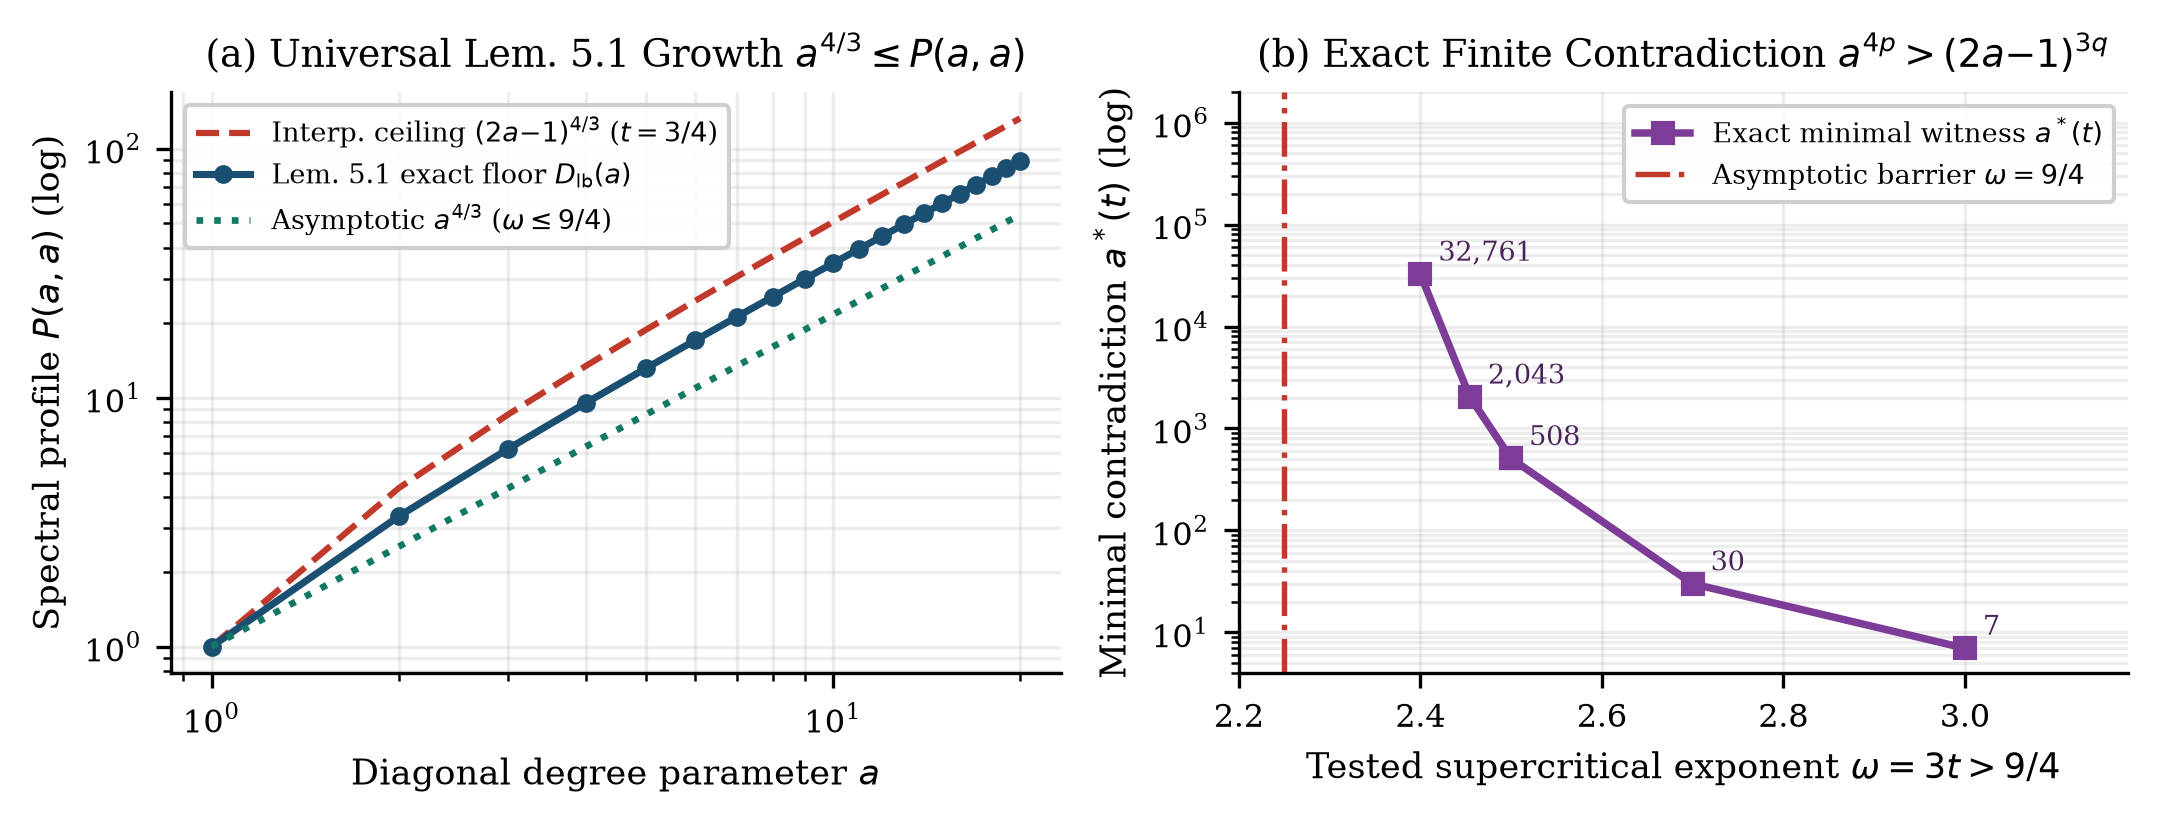
\includegraphics[width=\columnwidth]{figures/fig1_lemma51_growth_and_refutation.png}
\vspace{-1.4em}
\caption{\textbf{(a)}~Exact Lemma~5.1 diagonal lower envelope $D_{\mathrm{lb}}(a) = \frac{3a-1}{2}\prod_{m=1}^{a-1}(1+\frac{1}{3m})$ bounded strictly above $a^{4/3}$ and below the $t=3/4$ interpolation ceiling $(2a-1)^{4/3}$ for $a\ge 2$. \textbf{(b)}~Exact minimal integer contradiction witnesses $a^*(t)$ where $a^{4p}>(2a-1)^{3q}$ refutes supercritical $\omega=3t>9/4$ ($a^*=7$ at $\omega=3$ up to $32{,}761$ at $\omega=12/5$).}
\label{fig:lem51}
\end{figure}

\begin{figure}[t]
\centering
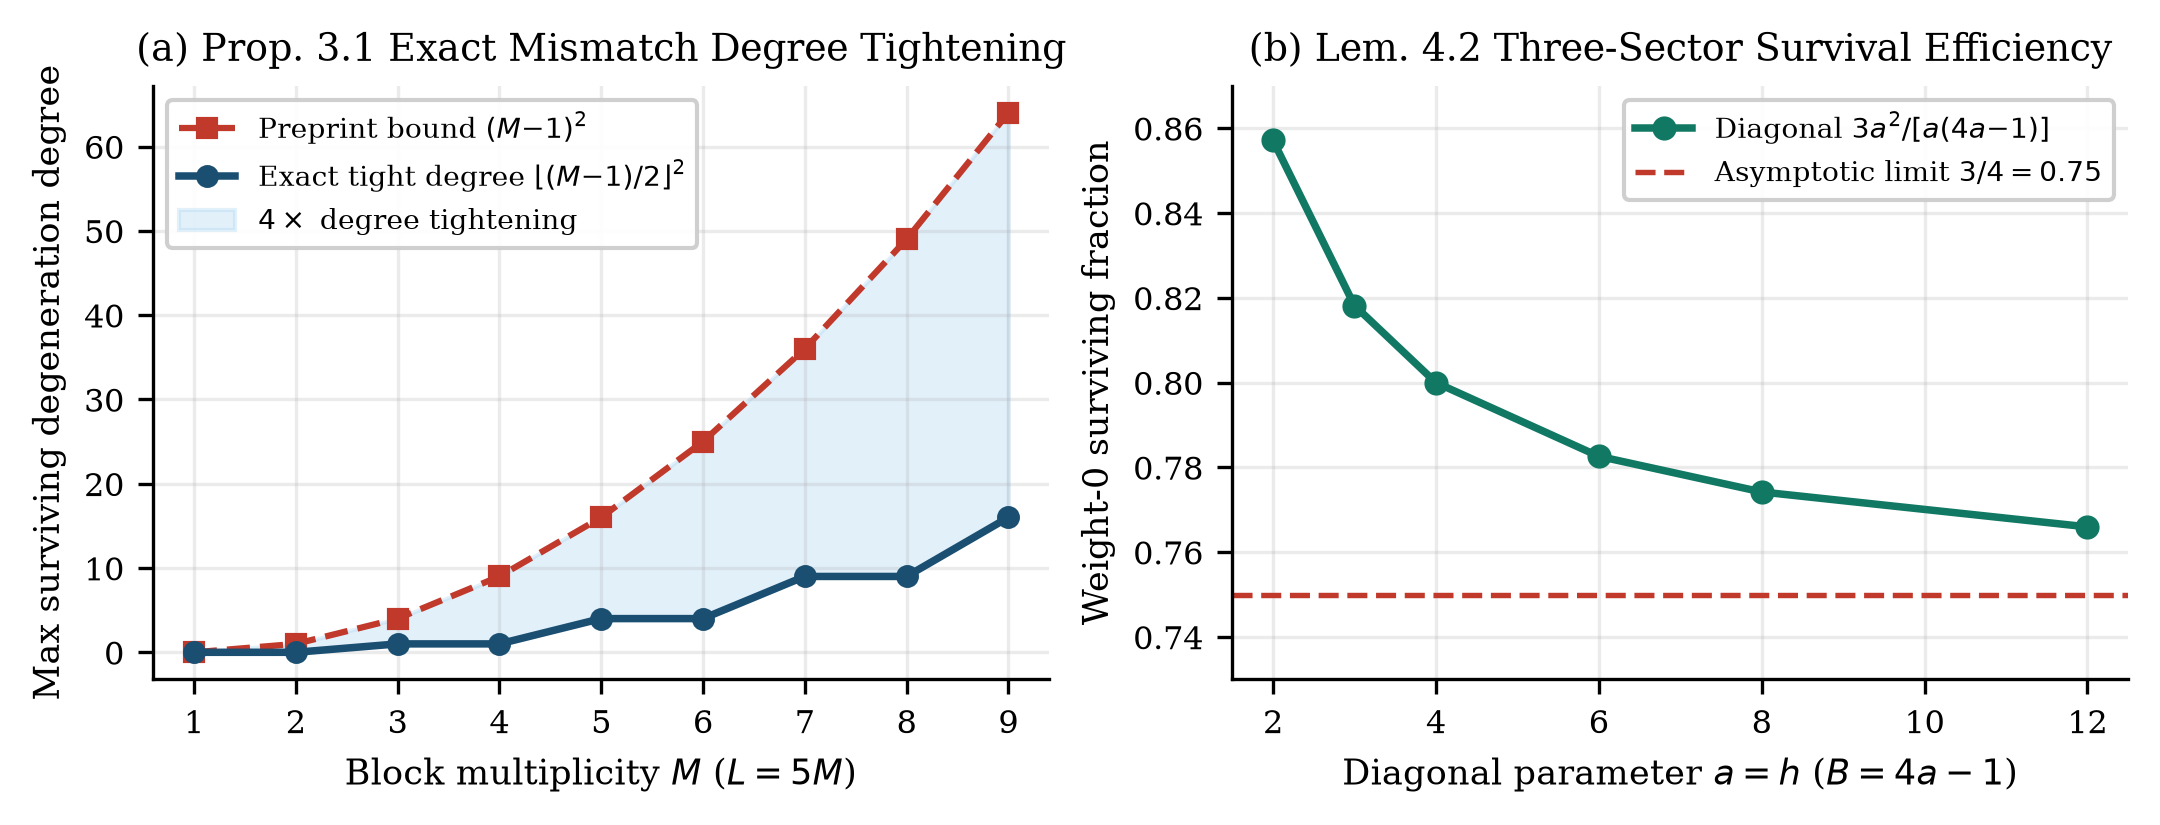
\includegraphics[width=\columnwidth]{figures/fig2_prop31_and_lem42.png}
\vspace{-1.4em}
\caption{\textbf{(a)}~Sharp $4\times$ tightening of Proposition~3.1's surviving degeneration degree from $(M-1)^2$ to $\lfloor(M-1)/2\rfloor^2$ across $M\in[1,9]$. \textbf{(b)}~Lemma~4.2 diagonal three-sector weight-$0$ survival fraction $\frac{3a}{4a-1}$ converging monotonically to $3/4$.}
\label{fig:prop31}
\end{figure}

\section{Exact Findings, Atlas, and Red-Team Audit}\label{sec:exp}
All experiments ran locally on Windows~11 (Python~3.12.6, Lean~4.35.0; 7-run means after warm-up).

\paragraph{1. Sharp $4\times$ Tightening of Proposition~3.1 Degree (Fig.~\ref{fig:prop31}(a)).}
OpenAI~\cite{openai2026omega94upper} (p.~5) bounds the degree of the transformed tensor in Proposition~3.1 by $(M-1)^2$. Exhaustive exact auditing across $M=1,\dots,9$ reveals that because surviving terms satisfy $2(g-h) = v-u$ with $u,v\in\{1,\dots,M\}$, we necessarily have $|g-h| \le \lfloor(M-1)/2\rfloor$, tightening the maximum surviving weight by a factor of $4$ to $\lfloor(M-1)/2\rfloor^2$: at $M=2$ the actual maximum weight is $0$ (zero-degree exact restriction!), and at $M=8$ it is $9$ versus $49$.

\paragraph{2. Exact Matrix Factorization, Sector Survival, \& Finite Contradiction Witnesses (Figs.~\ref{fig:lem51}--\ref{fig:atlas}).}
In Mode~2, exact $\QQ$ matrix conjugation confirms zero upper-right entries across every slice $f_r \in V_{a-1}$ of $C(a,b)\otimes B_X(2)$, with exact diagonal nonzeros $a(b+1)$ and $a(b-1)$ and cross-block nonzeros equal to $a-1$ (e.g.\ $1$ for $C(2,2)$ matching $u(vw)=v^2s+vD$, and $5$ for $C(6,6)$). In Mode~3, $C(2,4)$ yields exactly $3\times 2=6$ weight-$0$ terms and $2$ dropped weight-$+1$ terms (matching Fig.~1 of~\cite{openai2026omega94upper}), and diagonal survival efficiency $\frac{3a}{4a-1}$ approaches $3/4$ (Fig.~\ref{fig:prop31}(b)). In Mode~4, we construct explicit rational spectral profiles—including the zero-slack tight profile $P_{1/3}(a,b) = a+b-1+\frac13(a-1)(b-1)$ (where $P(2,3h+1)=3P(2,h)$ holds with zero slack for every $h$) and strictly concave rational families $a+b-1+\alpha(a-1)(b-1)+\beta\frac{(a-1)(b-1)}{a+b+c}$ ($\beta>0$, $c\ge 0$, $3\alpha-1\ge 2\beta$)—and compute exact minimal finite contradiction thresholds $a^*(t)$ ruling out $\omega=3$ at $a^*=7$ ($7^4=2401>2197=13^3$, also certified in Lean Theorem~18 alongside the chain $2 < \frac94 < 2.371177 < \frac52 < \log_2 7 < 3$ comparing $\frac94$ to the prior best bound $2.371177$ cited in~\cite[Sec.~1]{openai2026omega94upper}), $\omega=27/10$ at $a^*=30$, $\omega=5/2$ at $a^*=508$, $\omega=27/11$ at $a^*=2{,}043$, and $\omega=12/5$ at $a^*=32{,}761$ (Fig.~\ref{fig:lem51}(b)).

\begin{figure}[t]
\centering
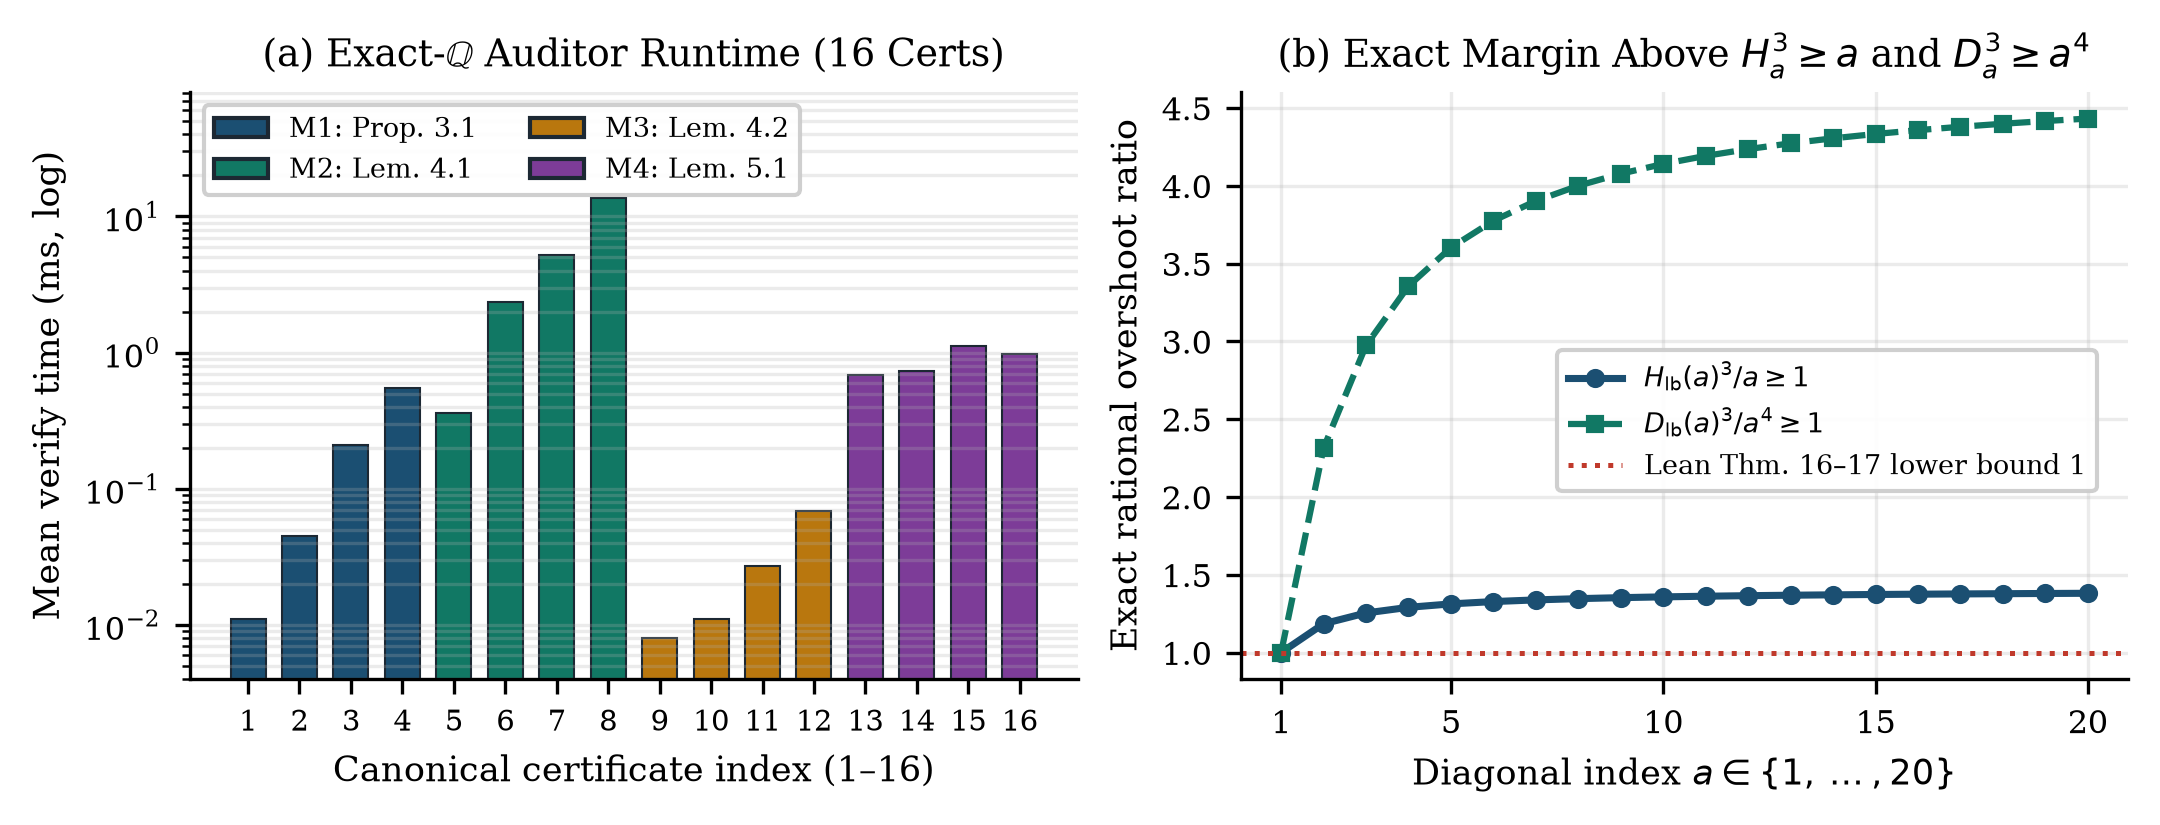
\includegraphics[width=\columnwidth]{figures/fig3_atlas_and_margins.png}
\vspace{-1.4em}
\caption{\textbf{(a)}~Mean exact-$\QQ$ verification latency across all 16 canonical certificates ($0.008$--$13.686\,\mathrm{ms}$). \textbf{(b)}~Exact rational overshoot ratios $H_{\mathrm{lb}}(a)^3/a \ge 1$ and $D_{\mathrm{lb}}(a)^3/a^4 \ge 1$ across $a\in\{1,\dots,20\}$.}
\label{fig:atlas}
\end{figure}

\paragraph{3. 16-Certificate Atlas \& 64-Check Red-Team Audit.}
Table~\ref{tab:atlas} summarizes all 16 canonical certificates verified in $0.008$--$13.686\,\mathrm{ms}$. \texttt{tests/test\_suite.py} executes 64 pytest checks (all passing in $0.13\,\mathrm{s}$): all 16 canonical certificates, 3 raw-JSON IEEE-754/\texttt{NaN}/duplicate-key parser rejections, and 60 live adversarial forgery attacks across schema/parser bypasses (12), Mode~1 (10), Mode~2 (12), Mode~3 (10), and Mode~4 (16). \texttt{scripts/verify\_all.py} enforces all 5 gates including a strict axiom whitelist and 40-file SHA-256 manifest.

\begin{table}[t]
\centering
\caption{Canonical 16-certificate \texttt{STRASSEN-94-CERT-1.0} atlas (\texttt{results/exp1\_certificate\_atlas.json}; all 16 verified).}
\label{tab:atlas}
\scriptsize
\setlength{\tabcolsep}{2.4pt}
\resizebox{\columnwidth}{!}{%
\begin{tabular}{@{}l c l r@{}}
\toprule
Certificate ID & M & Exact Certified Witness Summary & ms \\
\midrule
\texttt{prop31\_fourier\_M2\_base} & M1 & $M{=}2, L{=}10$, $4$ surv., $4$ w0, deg $0\le 1$ & 0.011 \\
\texttt{prop31\_fourier\_M4\_quartic} & M1 & $M{=}4, L{=}20$, $28$ surv., $16$ w0, deg $1\le 9$ & 0.045 \\
\texttt{prop31\_fourier\_M6\_hex} & M1 & $M{=}6, L{=}30$, $92$ surv., $36$ w0, deg $4\le 25$ & 0.210 \\
\texttt{prop31\_fourier\_M8\_octal} & M1 & $M{=}8, L{=}40$, $216$ surv., $64$ w0, deg $9\le 49$ & 0.553 \\
\texttt{lem41\_filtration\_C2\_2\_paper\_ex} & M2 & $C(2,2)$: $4{\to}6$, UR $0$, $*=1$, $+{=}6, -{=}2$ & 0.358 \\
\texttt{lem41\_filtration\_C3\_4\_asym} & M2 & $C(3,4)$: $8{\to}12$, UR $0$, $*=2$, $+{=}15, -{=}9$ & 2.343 \\
\texttt{lem41\_filtration\_C4\_5\_mid} & M2 & $C(4,5)$: $10{\to}16$, UR $0$, $*=3$, $+{=}24, -{=}16$ & 5.173 \\
\texttt{lem41\_filtration\_C6\_6\_square} & M2 & $C(6,6)$: $12{\to}22$, UR $0$, $*=5$, $+{=}42, -{=}30$ & 13.686 \\
\texttt{lem42\_sectors\_C2\_4\_fig1} & M3 & $a{=}2,h{=}1,B{=}4$: $3{\times}2$ w0, $2$ drop, $0$ neg & 0.008 \\
\texttt{lem42\_sectors\_C3\_8\_tripled} & M3 & $a{=}3,h{=}2,B{=}8$: $3{\times}6$ w0, $6$ drop, $0$ neg & 0.011 \\
\texttt{lem42\_sectors\_C5\_16\_mid} & M3 & $a{=}5,h{=}4,B{=}16$: $3{\times}20$ w0, $20$ drop & 0.027 \\
\texttt{lem42\_sectors\_C8\_31\_diag} & M3 & $a{=}8,h{=}8,B{=}31$: $3{\times}64$ w0, $56$ drop & 0.069 \\
\texttt{lem51\_profile\_tight\_alpha1\_3} & M4 & $a_{\max}{=}6$, $D_6{=}\frac{58}{3}$, refutes $t{=}1$ ($a{=}8$) & 0.686 \\
\texttt{lem51\_profile\_strict\_concave\_1\_2} & M4 & $a_{\max}{=}6$, $105$ strict conc., ref.\ $t{=}\frac56$ ($10^3$) & 0.728 \\
\texttt{lem51\_profile\_product\_ab\_amax8} & M4 & $a_{\max}{=}8$, $D_8{=}64$, refutes $t{=}\frac45$ ($5{\cdot}10^4$) & 1.121 \\
\texttt{lem51\_profile\_concave\_tight\_amax7} & M4 & $a_{\max}{=}7$, $150$ strict conc., ref.\ $t{=}\frac{9}{11}$ ($2048$) & 0.984 \\
\bottomrule
\end{tabular}}
\end{table}

\section{Conclusion}\label{sec:conc}
We delivered an independent, zero-dependency, zero-floating-point verification stack for OpenAI's $\omega\le 9/4$ Strassen spectral profile proof~\cite{openai2026omega94upper}, pairing 18 constructive Lean~4.35.0 theorems (including the complete universal inductive proof of Lemma~5.1, $P(a,a)^3\ge a^4$ for all $a\ge 1$, with zero \texttt{Classical.choice}) with the exact-$\QQ$ auditor \texttt{STRASSEN-94-CERT-1.0}, 16 canonical witnesses, a $4\times$ tightening of Proposition~3.1's degeneration degree, exact minimal finite refutation thresholds $a^*(t)$, and 60/60 live adversarial forgery rejections.

\bibliographystyle{plain}
\bibliography{references}
\end{document}
